%%Localization (chpt4)
\chapter{Localization} %5
The first of the two main ingredients of SLAM is localization. The task of localization is the estimation of the drone's position given a map and sensor information. In our case, the map is a map of visual features, and the main sensor used will be the camera. This part was already carried out by last year's groups, and it is already made to work in the three dimensional case. For completeness, we quickly repeat in this chapter how it works.

\section{Perspective-$n$-Point}\label{sec:pnp}
To localize the drone using visual information and a map, we need to solve the perspective-$n$-point (PnP) problem. PnP is the problem of estimating the six degrees of freedom 3D pose of a camera, given $n$ observations of 3D points whose locations are known. We use two main methods to solve the PnP problem: P3P and EPnP.

\subsection{P3P}
\begin{figure}[H]
\centering
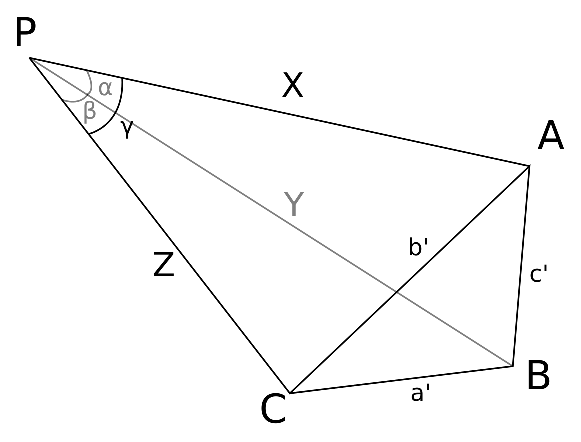
\includegraphics[width=0.3\textwidth]{p3p.eps}
\caption{Triangles in P3P}
\label{fig:p3p}
\end{figure}
The smallest number of point correspondences required to solve the PnP problem is 3, in which case it is called P3P. P3P can be solved with a method based on the cosine law, but it can have multiple solutions. A fourth point correspondence can be used to solve this uncertainty. Given three known points $A$, $B$ and $C$, and the center of projection of the camera $P$, define the following distances: $|A B| = c'$, $|B C| = a'$, $|C A| = b'$, $|P A| = X$, $|P B| = Y$, $|P C| = Z$, and the following angles: $\widehat{APB} = \alpha$, $\widehat{BPC} = \beta$, $\widehat{CPA} = \gamma$ (see figure \ref{fig:p3p}). We can then use the cosine law on each of the triangles that has $P$ and two of the points $A$, $B$, $C$ as vertices to obtain the following system of equations:
\begin{align}
  X^2 + Y^2 - XY\cdot2\cos(\alpha) - c'^2 &= 0 \\
  Y^2 + Z^2 - YZ\cdot2\cos(\beta)  - a'^2 &= 0 \\
  Z^2 + X^2 - ZX\cdot2\cos(\gamma) - b'^2 &= 0
\end{align}
The only unknowns is these equations are $X$, $Y$ and $Z$, as the distances between points $A$, $B$, $C$ can be deduced from their known position, and the angles can be deduced from the observations of these points on the image. For the resolution of these equations, the reader is referred to the paper that established the P3P method \cite{p3p}. As they show, it is possible to eliminate one of these equations and one of the variables to end up with two quadratic equations and two unknowns. This means that if there exists a finite number of solutions, that number has to be less than or equal to 4. To eliminate the bad solutions, a fourth point correspondence is used. Once $X$, $Y$ and $Z$ are determined, the position and orientation of point $P$ be can be deduced.

\subsection{EPnP}
EPnP (Efficient PnP) \cite{epnp} is a method to solve the more general PnP problem. It uses $n \geq 4$ point correspondences to estimate the position of the camera. The central idea of this method is to express the $n$ points as a weighted sum of four virtual points. Because it uses more points, it is more stable and resistant to noise than P3P.

\subsection{Random Sample Consensus}
Our data is subject to noise and measurement errors, which can negatively impact our solution. Do deal with this problem, we use Random Sample Consensus (RANSAC). RANSAC is a method to estimate parameters using data that contains outliers. The general idea is to iteratively estimate the parameters using different random samples, and to use a voting scheme to select the best parameters. The algorithm works in two steps:
\begin{enumerate}
  \item A random sample is drawn from the data with the smallest required number of examples to estimate model parameters. From this random sample, we estimate the parameters.
  \item We test all the data against the model estimated in step 1. All the data that whose loss according to some predefined loss function falls below a certain threshold when fitted to the model is considered part of the consensus set.
\end{enumerate}
Both above steps are repeated, and the model with the largest consensus set is selected. All the data that are part of this consensus set are considered to be inliers, and the rest of the data are considered outliers. A final model can then be computed using all inliers \cite{ransac}.\\

Applying this scheme to the PnP problem, we use the P3P method to create a model from each of the random samples, and then use the EPnP method on the inliers. This way we determine what points are outliers with the fastest method (P3P), and then use EPnP so that all inliers are used for the final estimation.

\section{Internal Pose Estimation}
As we said in section \ref{sec:closedsource}, the Parrot's closed-source code does not give us access to the individual sensor readings, but gives us the output of its own pose fusion. The information given is:
\begin{itemize}
\item The linear speed in all three directions (obtained by fusing the speed estimate from visual flow of the bottom camera and from integration of the accelerometers),
\item The three orientation angles (obtained by fusing the integrated rotational speed of the gyroscopes, an estimate of the gravity direction from the accelerometers, and the magnetometer)
\item The altitude (from the ultrasound sensor)
\end{itemize}
Of this information, the altitude and the roll and pitch angles are very accurate and drift-free. The other measurements are either speed estimates that have to be integrated, or the result of integration themselves. As a result, they are subject to drift, so while they are useful to stabilize the drone, they can't be used as an absolute reference.

\subsection{Visual Odometry from optical flow of the bottom camera} \label{sec:opticalflow}
Using the output of the bottom-facing camera, it is possible to deduce the ground speed of the drone. Because monocular camera measurements always give information only up to a scale factor, this only gives the ratio between altitude and speed. However, using the ultrasound sensor, that also points downwards, we know the altitude of the drone and can deduce its absolute ground speed. This visual odometry is already implemented by the constructor of the drone, as it is used to control the velocity of the drone during normal (remote-controlled) use. Unfortunately, the code that computes this velocity from the optical flow is part of the closed-source firmware, so we only have access to its output and have to use it as a black box.

\section{Pose Fusion}\label{sec:posefusion}
To obtain a final pose estimation, we will combine our estimation based on PnP and the estimation we receive from the drone. Our objective in doing so is for each source of information to compensate the shortcomings of the other ones:
\begin{itemize}
\item The result of PnP gives an estimate that is absolute with respect to the map, so the errors don't accumulate. However, because of the computations required to estimate the pose visually, estimates are not available frequently enough for the controller to efficiently stabilize the drone. Also, if the drone temporarily loses track of the map, this method gives no information at all
\item The various sensor readings are available at a high frequency, but most of them only directly measure acceleration or rotational speed, and have to be integrated to give an estimate of the position and orientation. For this reason, errors accumulate over time, leading the drone to drift away. The exception to this is the ultrasonic sensor, which gives an absolute measurement of the altitude. Deducing the gravitational direction from the accelerometer readings also gives a good measure of the roll and pitch angles.
\end{itemize}
To use the best characteristics of both estimates, we use the simple pose fusion algorithm that was developed by last year's group:
\begin{itemize}
\item We use the altitude from the ultrasound sensor, and the roll and pitch angles from the IMU directly.
\item Every time we receive an update of the visual pose estimation, we use it directly for the $x$, $y$ and yaw estimates
\item In between visual pose estimations, we use the position estimated by integrating the accelerometer and gyroscope data, integrating from the last visual pose.
\item To account for the possible delay between when the drone sees an image and when we can estimate the pose using PnP, we save the displacement between each successive pose estimation along with their respective times in a queue, and add all displacements that happened since the image was seen to the visual estimation obtained from that image.
\end{itemize}

\section{Summary}
The localization task is carried out by pose estimation node, using the output of the sensors, and the result of PnP, which is computed by the mapping node. When the mapping node receives a frame (list of keypoints) from the computer vision node, it matches the descriptors of this frame with the ones of the map, and uses these correspondences to estimate the pose visually, as explained in section \ref{sec:pnp}. The pose estimation node then uses the most recent visual pose estimate along with the speeds estimated from sensor readings, such as the speed estimated from optical flow (section \ref{sec:opticalflow}) to obtain a fused pose estimate, as explained in section \ref{sec:posefusion}. This pose fusion is quite rudimentary, and could significantly be improved, for example by using an extended Kalman filter, such as in \cite{engel2011msc}.\\

Figure \ref{fig:locflowchart} summarizes the localization part of the code in the form of a flowchart. It should be noted that only the pose fusion is carried out by the pose estimation node, the pose estimation using the map is carried out by the mapping node, as it is the node containing the map.
\begin{figure}[H]
\centering
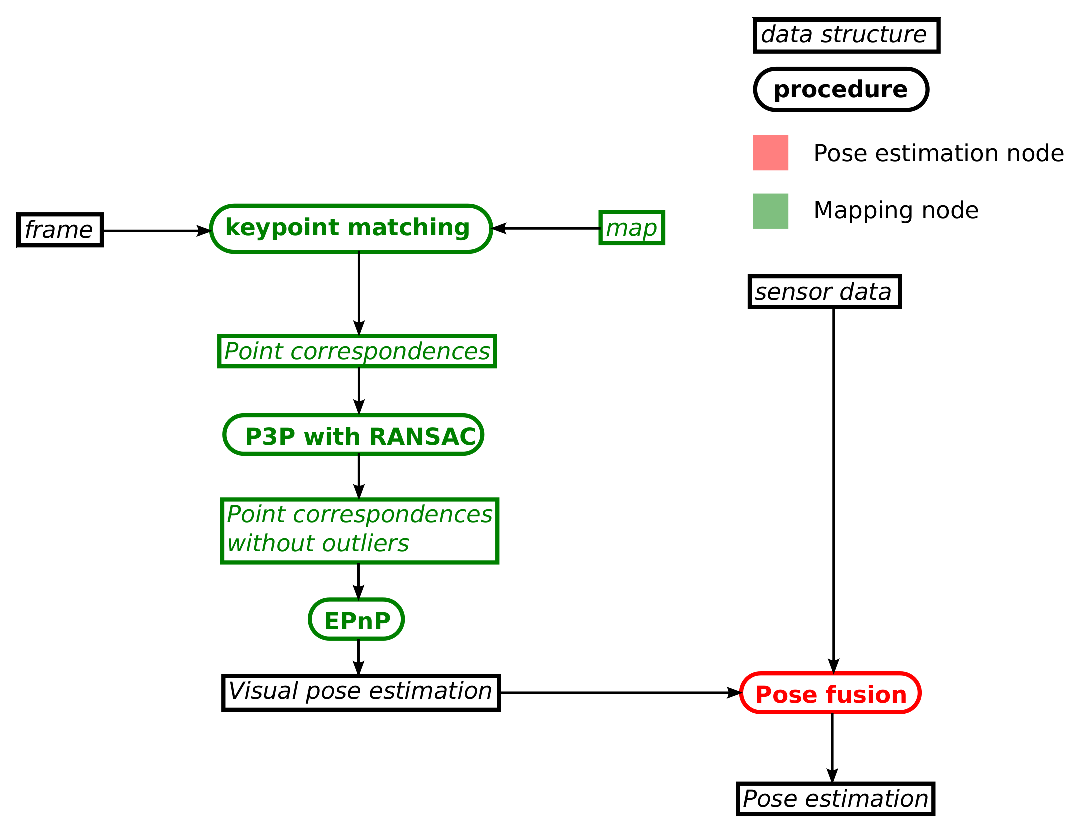
\includegraphics[width=\linewidth]{locflowchart.eps}
\caption{Flowchart of localization task}
\label{fig:locflowchart}
\end{figure}
